\documentclass[tikz,border=4pt]{standalone}
\usepackage{amsmath}
\usepackage{xcolor}
\usetikzlibrary{arrows.meta,positioning,calc}

\definecolor{ink}{HTML}{19232C}
\definecolor{subink}{HTML}{5B6872}
\definecolor{canvas}{HTML}{F8FAFC}
\definecolor{green}{HTML}{168A50}
\definecolor{greenbg}{HTML}{F2FBF5}
\definecolor{blue}{HTML}{2767D4}
\definecolor{bluebg}{HTML}{F2F6FD}
\definecolor{orange}{HTML}{D97706}
\definecolor{orangebg}{HTML}{FFF8F0}
\definecolor{red}{HTML}{D83C48}
\definecolor{purple}{HTML}{A45BD4}
\definecolor{grayedge}{HTML}{77838D}
\newcommand{\vect}[1]{\boldsymbol{#1}}

\begin{document}
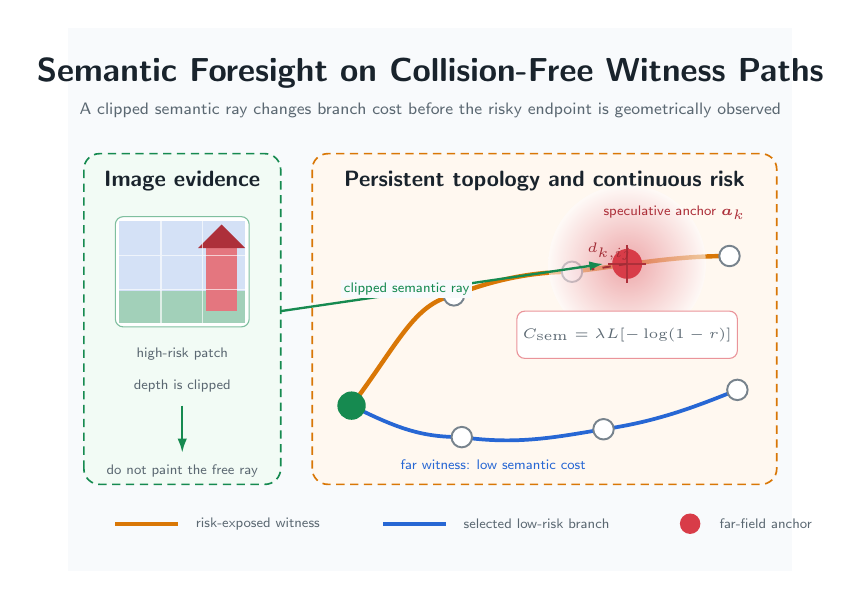
\begin{tikzpicture}[
  x=1mm,y=1mm,font=\sffamily,
  title/.style={font=\sffamily\bfseries\fontsize{13}{15}\selectfont,text=ink},
  subtitle/.style={font=\sffamily\fontsize{6.4}{8}\selectfont,text=subink},
  group/.style={font=\sffamily\bfseries\fontsize{8}{10}\selectfont,text=ink},
  note/.style={font=\sffamily\fontsize{5.2}{6.6}\selectfont,text=subink,align=center},
  panel/.style={rounded corners=2mm,line width=.6pt,dashed,dash pattern=on 3pt off 2pt},
  arrow/.style={-{Latex[length=1.8mm,width=1.2mm]},line width=.85pt},
  edge/.style={draw=grayedge!68,line width=.75pt},
  witness/.style={draw=orange,line width=1.6pt}
]
\fill[canvas] (-2,-4) rectangle (90,65);
\node[title] at (44,59.2) {Semantic Foresight on Collision-Free Witness Paths};
\node[subtitle] at (44,54.5) {A clipped semantic ray changes branch cost before the risky endpoint is geometrically observed};

% Observation panel
\filldraw[panel,fill=greenbg,draw=green] (0,7) rectangle (25,49);
\node[group] at (12.5,45.5) {Image evidence};
\filldraw[fill=white,draw=green!55,rounded corners=1mm] (4,27) rectangle (21,41);
\fill[blue!20] (4.5,27.5) rectangle (20.5,40.5);
\fill[green!40] (4.5,27.5) rectangle (20.5,31.5);
\fill[red!70] (15.5,29) rectangle (19.5,37);
\fill[red!80!black] (14.5,37) -- (17.5,40) -- (20.5,37) -- cycle;
\draw[white,opacity=.65] (9.8,27.5)--(9.8,40.5) (15.1,27.5)--(15.1,40.5)
  (4.5,31.8)--(20.5,31.8) (4.5,36.1)--(20.5,36.1);
\node[note] at (12.5,23.5) {high-risk patch};
\node[note] at (12.5,19.5) {depth is clipped};
\draw[arrow,draw=green] (12.5,17) -- (12.5,11);
\node[note] at (12.5,8.7) {do not paint the free ray};

% Topological scene panel
\filldraw[panel,fill=orangebg,draw=orange] (29,7) rectangle (88,49);
\node[group] at (58.5,45.5) {Persistent topology and continuous risk};

% two branches
\coordinate (s) at (34,17);
\coordinate (u1) at (47,31);
\coordinate (u2) at (62,34);
\coordinate (ut) at (82,36);
\coordinate (l1) at (48,13);
\coordinate (l2) at (66,14);
\coordinate (lt) at (83,19);
\draw[edge] (s) .. controls (40,25) and (42,30) .. (u1);
\draw[edge] (u1) .. controls (52,33) and (57,34) .. (u2);
\draw[edge] (u2) .. controls (70,35) and (75,36) .. (ut);
\draw[edge] (s) .. controls (40,14) and (43,13) .. (l1);
\draw[edge] (l1) .. controls (55,12) and (60,13) .. (l2);
\draw[edge] (l2) .. controls (73,15) and (78,17) .. (lt);

% witness overlays
\draw[witness] (s) .. controls (40,25) and (42,30) .. (u1)
  .. controls (52,33) and (57,34) .. (u2)
  .. controls (70,35) and (75,36) .. (ut);
\draw[blue,line width=1.35pt] (s) .. controls (40,14) and (43,13) .. (l1)
  .. controls (55,12) and (60,13) .. (l2)
  .. controls (73,15) and (78,17) .. (lt);

\foreach \p in {s,u1,u2,ut,l1,l2,lt}{\fill[white,draw=grayedge,line width=.7pt] (\p) circle (1.3mm);}
\fill[green] (s) circle (1.8mm);

% risk field and anchor
\shade[inner color=red!70,outer color=red!2,opacity=.62] (69,35) circle (10mm);
\fill[red] (69,35) circle (1.9mm);
\draw[red!80!black,line width=.75pt] (69,32.6)--(69,37.4) (66.6,35)--(71.4,35);
\node[note,text=red!80!black] at (75,41.5) {speculative anchor $\vect a_k$};
\draw[arrow,draw=green] (25,29) -- (66,35);
\node[note,text=green,fill=canvas,inner sep=1pt] at (41,31.8) {clipped semantic ray};
\draw[red!75!black,dashed,line width=.7pt] (69,35) -- (64.5,34.3);
\node[note,text=red!75!black] at (66.8,36.6) {$d_{k,ij}$};

% branch labels and cost cards
\node[note,text=blue,anchor=west] at (39,9.5) {far witness: low semantic cost};
\filldraw[fill=white,draw=red!55,rounded corners=1mm] (55,23) rectangle (83,29);
\node[note] at (69,26) {$C_{\rm sem}=\lambda L[-\log(1-r)]$};

% Legend
\draw[witness] (4,2) -- (12,2); \node[note,anchor=west] at (13,2) {risk-exposed witness};
\draw[blue,line width=1.35pt] (38,2) -- (46,2); \node[note,anchor=west] at (47,2) {selected low-risk branch};
\fill[red] (77,2) circle (1.3mm); \node[note,anchor=west] at (79.5,2) {far-field anchor};
\end{tikzpicture}
\end{document}
